%%% Co-training.tex --- 
%% Version: $Id: Co-training.tex,v 0.0 2012/05/14 03:14:46 tangboyun Exp$
%% Copyright : (c) 2012 Boyun Tang
%% License : BSD-style
\documentclass{standalone}
\usepackage{tikz}
\usetikzlibrary{mindmap,shadows,shapes.arrows,shapes.geometric,shapes.misc,matrix,arrows,positioning,calc,decorations.pathreplacing,petri}
\usepackage{graphicx}
\usepackage{times}
\usepackage{xcolor}
\begin{document}

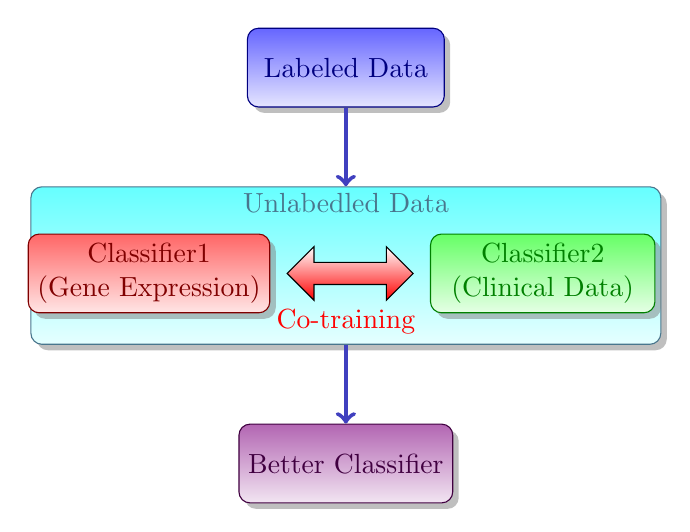
\begin{tikzpicture}[
  every node/.style={minimum width=2.5cm,minimum height=1cm,align=center,},%
  dr/.style={drop shadow},%
  e/.style={->,ultra thick,rounded corners,draw=blue!50!gray},%
  cl/.style={cylinder,aspect=.3,shape border rotate=90,},%
  re/.style={rounded corners,},%
  r/.style={top color= red!60,bottom color= red!10,draw=red!50!black,%
    text=red!50!black,},%
  g/.style={top color= green!60,bottom color= green!10,draw=green!50!black,%
    text=green!50!black,},%
  b/.style={top color= blue!60,bottom color= blue!10,draw=blue!50!black,%
    text=blue!50!black,},%
  br/.style={top color= brown!60,bottom color= brown!10,draw=brown!50!black,%
    text=brown!50!black,},%
  v/.style={top color= violet!60,bottom color= violet!10,draw=violet!50!black,%
    text=violet!50!black,},%
  o/.style={top color= orange!60,bottom color= orange!10,draw=orange!50!black,%
    text=orange!50!black,},%
  ye/.style={top color= yellow!60,bottom color= yellow!10,draw=yellow!50!black,%
    text=yellow!50!black,},%
  p/.style={top color= pink!60,bottom color= pink!10,draw=pink!50!black,%
    text=pink!50!black,},%
  c/.style={top color= cyan!60,bottom color= cyan!10,draw=cyan!50!black,%
    text=cyan!50!black,},%
  a/.style={double arrow,draw,bottom color=red,top color=white,shape border uses incircle,
    minimum height=2cm,minimum width=0.1cm,scale=.8}
  ]
  \node (la) [dr,re,b] {Labeled Data};
  \node (ul) [dr,re,c,minimum width=8cm,minimum height=2cm,below=of la] {};
  \node (ulf) [below=of la,yshift=0.3cm,text=cyan!50!black] {Unlabedled Data};
  \node (cl1) [dr,re,r,below=of la,xshift=-2.5cm,yshift=-.6cm] {Classifier1\\(Gene Expression)};
  \node (cl2) [dr,re,g,below=of la,xshift=2.5cm,yshift=-.6cm,minimum width=2.85cm] {Classifier2\\(Clinical Data)};  
  \node (co) [below=of ulf,text=red,yshift=0.5cm] {Co-training};
  \node (bc) [below=of ul,v,dr,re] {Better Classifier};
  \path (cl1) -- (cl2) node [a,midway] {};
  \draw [e] (la) -- (ul);
  \draw [e] (ul) -- (bc);
\end{tikzpicture}
\end{document}

%%% Local Variables: 
%%% TeX-master: t
%%% End: 
